% ======================================================================
% Qwen3.5-9B Four-Agent OODA Orchestration Framework (Version 1.0)
% Founder-Grade Whitepaper (Investor + Technical Partner + Engineer Ready)
% Single-file, compile-ready LaTeX document (.tex)
%
% Build (recommended):
%   latexmk -pdf -interaction=nonstopmode -halt-on-error whitepaper.tex
%
% Alternative (XeLaTeX):
%   latexmk -xelatex -interaction=nonstopmode -halt-on-error whitepaper.tex
%
% Notes:
% - This file is designed to compile under pdfLaTeX OR XeLaTeX.
% - Model download URLs and certain environment details are intentionally
%   left as placeholders per requirements.
% - Citations are included as placeholders and primary-source references.
% - macOS version / MLX versions are left unspecified unless stated in
%   cited upstream docs. Add exact pinning in Appendix if desired.
% ======================================================================

\documentclass[11pt]{article}

% -------------------------- Engine Compatibility -----------------------
\usepackage{iftex}
\ifPDFTeX
  \usepackage[T1]{fontenc}
  \usepackage[utf8]{inputenc}
  \usepackage{lmodern}
\else
  \usepackage{fontspec}
  % Choose a widely-available font set (TeX Live / MacTeX friendly):
  \setmainfont{TeX Gyre Pagella}
  \setsansfont{TeX Gyre Heros}
  \setmonofont{TeX Gyre Cursor}
\fi

% -------------------------- Layout / Typography ------------------------
\usepackage[margin=1in]{geometry}
\usepackage{microtype}
\usepackage{setspace}
\setstretch{1.07}

\usepackage{graphicx}
\usepackage{xcolor}
\usepackage{hyperref}
\usepackage{xurl}
\usepackage{url}
\usepackage{bookmark}

\hypersetup{
  colorlinks=true,
  linkcolor=blue!60!black,
  citecolor=blue!60!black,
  urlcolor=blue!50!black,
  pdftitle={Qwen3.5-9B Four-Agent OODA Orchestration Framework (Version 1.0)},
  pdfauthor={\textit{[Organization / Author Placeholder]}},
  pdfsubject={Local Agent Orchestration on Apple Silicon with MLX},
  pdfkeywords={agents, OODA, MLX, Qwen3.5, orchestration, local AI}
}

\usepackage{amsmath, amssymb}
\usepackage{enumitem}
\setlist[itemize]{leftmargin=*, itemsep=4pt, topsep=6pt}
\setlist[enumerate]{leftmargin=*, itemsep=4pt, topsep=6pt}

\usepackage{booktabs}
\usepackage{tabularx}
\usepackage{longtable}
\usepackage{multirow}
\usepackage{siunitx}
\sisetup{detect-all=true}

\usepackage{float}
\usepackage{caption}
\usepackage{subcaption}

\usepackage{tikz}
\usetikzlibrary{arrows.meta, positioning, shapes.geometric, shapes.misc, fit, calc}

\usepackage{listings}
\usepackage{tcolorbox}
\tcbuselibrary{breakable}

% -------------------------- Document Macros ----------------------------
\newcommand{\FrameworkName}{Qwen3.5-9B Four-Agent OODA Orchestration Framework}
\newcommand{\FrameworkVersion}{Version 1.0}
\newcommand{\TargetHardware}{Apple Silicon Mac mini (32\,GB unified memory, 1\,TB storage)}
\newcommand{\DateIssued}{March 2026}
\newcommand{\CoreModel}{\texttt{mlx-community/Qwen3.5-9B-MLX-8bit} (or 4-bit for headroom)}
\newcommand{\OptionalSynthesisModel}{\texttt{mlx-community/Qwen3.5-27B-4bit} or \textit{[larger fitting local model]}}
\newcommand{\Confidentiality}{\textit{[Public / Confidential]}} % Adjust as needed.

% -------------------------- Listings Styles ----------------------------
\definecolor{CodeBG}{rgb}{0.97,0.97,0.98}
\definecolor{CodeFrame}{rgb}{0.85,0.85,0.88}

\lstdefinestyle{base}{
  backgroundcolor=\color{CodeBG},
  frame=single,
  rulecolor=\color{CodeFrame},
  frameround=tttt,
  framesep=6pt,
  basicstyle=\ttfamily\small,
  breaklines=true,
  breakatwhitespace=false,
  showstringspaces=false,
  tabsize=2,
  numbers=left,
  numberstyle=\tiny,
  numbersep=8pt,
  captionpos=b
}

\lstdefinestyle{python}{
  style=base,
  language=Python,
  morekeywords={Path, Optional, Dict, List, Tuple, Union, dataclass},
  keywordstyle=\color{blue!60!black},
  commentstyle=\color{black!55},
  stringstyle=\color{teal!60!black}
}

\lstdefinestyle{json}{
  style=base,
  language={},
  keywordstyle=\color{blue!60!black},
  commentstyle=\color{black!55},
  stringstyle=\color{teal!60!black}
}

% -------------------------- Callout Boxes ------------------------------
\newtcolorbox{InvestorBox}{
  enhanced,
  breakable,
  colback=blue!3,
  colframe=blue!35!black,
  title=\textbf{Investor Takeaway},
  fonttitle=\bfseries,
  arc=2mm,
  boxrule=0.6pt
}

\newtcolorbox{EngineeringBox}{
  enhanced,
  breakable,
  colback=black!2,
  colframe=black!30,
  title=\textbf{Engineering Note},
  fonttitle=\bfseries,
  arc=2mm,
  boxrule=0.6pt
}

\newtcolorbox{AssumptionsBox}{
  enhanced,
  breakable,
  colback=yellow!8,
  colframe=yellow!45!black,
  title=\textbf{Assumptions \& Placeholders},
  fonttitle=\bfseries,
  arc=2mm,
  boxrule=0.6pt
}

% -------------------------- Title Metadata -----------------------------
\title{\FrameworkName\\\large \FrameworkVersion\ --- Founder-Grade Whitepaper}
\author{\textit{[Author / Team Name Placeholder]}\\\textit{[Company Placeholder]}\\\textit{[Contact Placeholder]}}
\date{\DateIssued}

% ======================================================================
\begin{document}

% -------------------------- Title Page ---------------------------------
\begin{titlepage}
  \centering
  \vspace*{1.0cm}

  % --- Logo Placeholder ---
  % \includegraphics[width=0.25\textwidth]{figures/logo.png} % <- Insert logo here
  \vspace{1.0cm}

  {\Huge\bfseries \FrameworkName \par}
  \vspace{0.2cm}
  {\Large \FrameworkVersion \par}

  \vspace{0.6cm}
  {\large Targeted Deployment: \TargetHardware \par}

  \vspace{0.4cm}
  {\large Core Model Substrate: \CoreModel \par}
  {\large Optional Final Synthesis: \OptionalSynthesisModel \par}

  \vfill

  \begin{tcolorbox}[colback=black!2, colframe=black!25, arc=2mm, boxrule=0.6pt, width=0.92\textwidth]
    \textbf{Document Classification:} \Confidentiality\\
    \textbf{Purpose:} Investor-ready and engineering-credible specification of a local-first, guardrailed, multi-agent orchestration system built around an OODA-inspired workflow (Observe--Orient--Decide--Act).\\
    \textbf{Disclaimer:} This document is for informational purposes and does not constitute investment advice.
  \end{tcolorbox}

  \vspace{0.8cm}
  {\large \DateIssued \par}
  \vspace{0.4cm}
  {\small \textit{Prepared by: [Author/Org Placeholder]}\par}

\end{titlepage}

\pagenumbering{roman}

% -------------------------- Executive Summary --------------------------
\section*{Executive Summary}
\addcontentsline{toc}{section}{Executive Summary}

\FrameworkName\ is a \textbf{local-first cognitive orchestration layer} designed to run entirely on Apple Silicon hardware using MLX and MLX-LM---Apple's open-source stack for efficient machine learning and LLM workflows on Mac-class devices \cite{MLX_GitHub, MLX_Docs, MLXLM_Readme}.
It converts raw user requests into validated plans, strict intermediate specifications, and high-quality deliverables \textbf{without relying on cloud inference}, enabling privacy, low-latency iteration, and on-device execution.

\begin{InvestorBox}
\textbf{Why it matters:} Contemporary AI assistants are optimized for \emph{immediate answer generation} but frequently underperform at \emph{transformation integrity}: preserving intent, documenting assumptions, verifying reductions, and acting safely in real environments.
\FrameworkName\ solves this by enforcing a disciplined OODA pipeline and by representing all internal transformations as auditable state transitions (prompt $\rightarrow$ elevated prompt $\rightarrow$ discoveries $\rightarrow$ reduced spec $\rightarrow$ verified outputs).
\end{InvestorBox}

\noindent\textbf{Core innovation:} \textbf{one shared model substrate, four operational identities.}
All four agents run on the exact same local base model weights (e.g., Qwen3.5-9B in MLX format) while diverging only through system-prompt overlays, phase priority, and orchestration routing.
This design yields consistent behavior, a clean fine-tuning story, and lower runtime overhead compared to multi-model ensembles.

\noindent\textbf{Target platform:} \TargetHardware.
MLX provides a unified memory model in which arrays live in shared memory and can be operated on by CPU/GPU without explicit data transfers, which is especially relevant for on-device LLM inference \cite{MLX_GitHub, MLX_Docs}.

\noindent\textbf{Key capabilities:}
\begin{itemize}
  \item \textbf{OODA pipeline enforcement:} Every task follows Observe--Orient--Decide--Act, with mandatory prompt elevation, planning, consolidation, and verified execution.
  \item \textbf{Traceability by default:} All transformations are logged to an internal JSON trace for audit, reproducibility, and fine-tuning dataset creation.
  \item \textbf{Tag-driven outputs:} Users specify deliverables via tags (e.g., \texttt{[code][architecture-doc][summary]}). The system plans once, then renders multiple artifacts sequentially from the same validated specification.
  \item \textbf{Guardrailed local execution:} Terminal and filesystem tool access is scoped to user-approved directory roots, preventing unintended file modification outside the permitted sandbox.
  \item \textbf{Extensible specialization:} Fine-tuning via LoRA/QLoRA is supported through MLX-LM's training workflow (adapter-based specialization) \cite{MLXLM_LoRA}.
\end{itemize}

\vspace{6pt}
\noindent\textbf{Bottom line:} \FrameworkName\ is positioned as a \textbf{private cognitive operating layer} for serious work: software engineering, structured research, technical writing, and execution-heavy workflows, with a high-integrity pipeline designed for investor confidence and engineering trust.

% -------------------------- Abstract -----------------------------------
\section*{Abstract}
\addcontentsline{toc}{section}{Abstract}

We present a production-oriented, local-first, four-agent orchestration framework that operationalizes the OODA loop (Observe--Orient--Decide--Act) for reliable AI-assisted work.
The system runs on Apple Silicon using MLX and MLX-LM, and uses a single shared Qwen3.5-9B MLX model instance to implement four dynamically routed agent identities.
Agents differ only by instruction overlays and invocation context, enabling consistent behavior and a straightforward fine-tuning path.

The framework enforces transformation integrity through a mandatory workflow:
(1) prompt elevation,
(2) exploration and planning,
(3) consolidation into formal specification with verification,
(4) guarded execution and multi-output generation, and
(5) optional final synthesis using a larger local model.
We define a traceability model (JSON state trace), a tag-driven output planner, a filesystem and subprocess safety model, and implementation-ready MLX Python code.

% -------------------------- Tables / TOC --------------------------------
\tableofcontents
\listoftables
\listoffigures
\newpage
\pagenumbering{arabic}

% ======================================================================
\section{Introduction: The Local Cognitive Operating Layer}

The market is transitioning from chat-based assistants to systems that can \emph{plan, verify, and act} in software and operational environments.
However, many current solutions lack deterministic process structure: the model generates early, assumptions remain implicit, and action systems (files, terminals) operate with weak or opaque control.
\FrameworkName\ proposes a disciplined local-first alternative.

\begin{EngineeringBox}
\textbf{Primary foundation:} MLX is an array framework for Apple Silicon with a unified memory model (arrays in shared memory; operations across supported devices without explicit data copies) \cite{MLX_GitHub, MLX_Docs}.
MLX-LM provides LLM generation and fine-tuning workflows on Apple Silicon and integrates Hugging Face model loading and quantization pipelines \cite{MLXLM_Readme}.
\end{EngineeringBox}

\subsection{Scope and Target Audience}

This whitepaper targets:
\begin{itemize}
  \item \textbf{Investors:} market positioning, differentiation, roadmap, and defensibility.
  \item \textbf{Technical partners:} integration concepts, guardrails, and deployment feasibility.
  \item \textbf{Engineers:} clear interfaces, contracts, code skeletons, and operational assumptions.
\end{itemize}

\subsection{Assumptions and Unspecified Details}

\begin{AssumptionsBox}
\begin{itemize}
  \item \textbf{macOS version:} Not specified. MLX-LM notes that certain large-model performance optimizations (model/cache memory ``wiring'') require macOS 15.0+ \cite{MLXLM_Readme}.
  \item \textbf{Exact Mac mini chip variant:} Not specified (e.g., M2 vs M2 Pro vs later). Performance estimates are therefore ranges, not guarantees.
  \item \textbf{Exact model URLs:} This document uses IDs and placeholders. Insert final download URLs in Appendix D.
  \item \textbf{MLX / MLX-LM versions:} Not pinned in this doc. Pin versions in deployment tooling for production (Appendix C).
\end{itemize}
\end{AssumptionsBox}

% ======================================================================
\section{Problem Statement}

AI assistants typically optimize for response fluency and breadth, but not for transformation integrity and safe actuation:
\begin{itemize}
  \item \textbf{Ambiguity propagation:} If a prompt is incomplete, the system often guesses rather than formalizes missing constraints.
  \item \textbf{Plan/output collapse:} Planning and rendering are conflated; downstream artifacts inherit unverified assumptions.
  \item \textbf{Weak auditability:} It is often unclear what the output is based on, what was discarded, and why.
  \item \textbf{Unsafe execution surfaces:} When terminals and files are involved, insufficient scoping can create unacceptable risk.
  \item \textbf{Cloud dependence:} Many high-capability systems assume remote inference; this introduces privacy, latency, and availability constraints.
\end{itemize}

\FrameworkName\ addresses these by making \emph{structured process} a first-class product feature.

% ======================================================================
\section{Thesis and Design Principles}

\subsection{Core Thesis}

\textbf{A single strong local model, orchestrated through disciplined multi-agent identities and verified workflow gates, can outperform ``single-pass'' assistants for real work.}
The performance driver is not only raw model capability; it is \emph{process structure, auditability, and controlled execution.}

\subsection{Principles}

\begin{itemize}
  \item \textbf{Unified architecture, adaptive specialization:} All agents share the same weights; differentiation is operational (instruction overlays and routing).
  \item \textbf{OODA embedded:} Every request follows Observe--Orient--Decide--Act.
  \item \textbf{Mixture-of-experts routing without multi-model overhead:} Specialist behavior is prompt-conditioned, not weight-conditioned.
  \item \textbf{Traceability and safety first:} Every transformation step is recorded in a trace object.
  \item \textbf{Tag-driven multi-output production:} Multiple deliverables are produced from a single verified plan.
  \item \textbf{Local-only execution:} Runs on-device using MLX/MLX-LM \cite{MLX_GitHub, MLXLM_Readme}.
\end{itemize}

\subsection{Why Qwen3.5 + MLX}

Qwen3.5 is a publicly released model family with multiple sizes (including 9B and 27B-class checkpoints) and emphasizes architectural efficiency and agentic capability \cite{Qwen35_GitHub, Qwen35_27B_Card, Qwen35_9B_BaseCard}.
MLX-LM provides generation, quantization, and fine-tuning (including LoRA/QLoRA) on Apple Silicon \cite{MLXLM_Readme, MLXLM_LoRA}.

% ======================================================================
\section{Technical Architecture}

\subsection{System Overview}

The system is composed of:
\begin{enumerate}
  \item \textbf{Base Model Runtime:} a single loaded Qwen3.5-9B MLX model instance (quantized).
  \item \textbf{Four Agent Identities:} instruction overlays enabling phase-specialized behavior.
  \item \textbf{Orchestrator:} a lightweight controller that enforces the OODA pipeline and routes tasks.
  \item \textbf{Tool Layer:} guarded filesystem and subprocess primitives.
  \item \textbf{Trace Store:} JSON trace capturing full transformation lineage.
\end{enumerate}

\subsection{Model Substrate and Local Inference Tooling}

\paragraph{MLX core.}
MLX is an Apple Silicon-focused ML framework with a unified memory model and multi-device execution \cite{MLX_GitHub, MLX_Docs}.

\paragraph{MLX-LM.}
MLX-LM is a Python package for generating text and fine-tuning LLMs on Apple Silicon with MLX, with Hugging Face Hub integration, quantization workflows, and LoRA/QLoRA support \cite{MLXLM_Readme, MLXLM_LoRA}.

\paragraph{Qwen3.5 support.}
Qwen documentation provides MLX-LM instructions and references converting models into MLX format using \texttt{mlx\_lm.convert} \cite{Qwen_MLXLM_Docs}.

\paragraph{MLX model availability.}
The MLX community publishes converted model checkpoints on Hugging Face \cite{MLXLM_Readme}.
A Qwen3.5-9B MLX 8-bit checkpoint is available as \texttt{mlx-community/Qwen3.5-9B-MLX-8bit} and includes quantization details and on-disk size \cite{MLXCommunity_Qwen35_9B_MLX8}.

\subsection{Agent Continuum and Routing}

\begin{figure}[H]
\centering
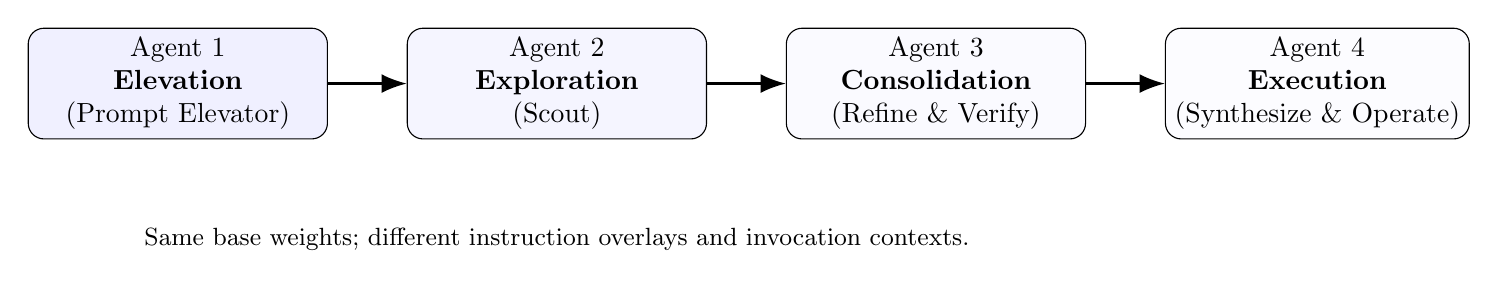
\begin{tikzpicture}[
  node distance=8mm and 10mm,
  box/.style={draw, rounded corners=2mm, align=center, minimum width=3.8cm, minimum height=1.0cm},
  arrow/.style={-{Latex[length=3.2mm]}, thick}
]
\node[box, fill=blue!6] (a1) {Agent 1\\\textbf{Elevation}\\(Prompt Elevator)};
\node[box, fill=blue!4, right=of a1] (a2) {Agent 2\\\textbf{Exploration}\\(Scout)};
\node[box, fill=blue!2, right=of a2] (a3) {Agent 3\\\textbf{Consolidation}\\(Refine \& Verify)};
\node[box, fill=blue!1, right=of a3] (a4) {Agent 4\\\textbf{Execution}\\(Synthesize \& Operate)};

\draw[arrow] (a1) -- (a2);
\draw[arrow] (a2) -- (a3);
\draw[arrow] (a3) -- (a4);

\node[align=center, below=10mm of a2] (note) {\small Same base weights; different instruction overlays and invocation contexts.};
\end{tikzpicture}
\caption{Operational continuum: one shared model substrate expressed as four phase-optimized agent identities.}
\label{fig:agent_continuum}
\end{figure}

\subsection{Traceability as a First-Class Primitive}

The orchestrator persists a trace object:
\begin{itemize}
  \item improves auditability and debugging,
  \item enables deterministic review,
  \item provides training data for iterative improvement and LoRA fine-tuning.
\end{itemize}

% ======================================================================
\section{Agent Specifications (Detailed Behaviors)}

All agents share the same base model runtime; primary differentiation is the system prompt overlay, output contracts, and routing policy.

\subsection{Agent 1 --- Elevation Agent (Prompt Elevator)}

\textbf{Mission:} Convert raw user intent into a complete, precise, verifiable problem statement.

\textbf{Non-negotiables:}
\begin{itemize}
  \item Must eliminate ambiguity or explicitly enumerate it.
  \item Must output \emph{only} the elevated prompt state in a structured format.
  \item Must define success criteria and constraints that downstream agents can verify.
\end{itemize}

\textbf{Input contract:} raw user request + optional tags.

\textbf{Output contract (recommended):}
\begin{itemize}
  \item Elevated prompt (single canonical statement).
  \item Explicit assumptions.
  \item Constraints / requirements.
  \item Acceptance tests / success criteria.
  \item Permissions requested (e.g., directory scope changes) if needed.
\end{itemize}

\textbf{Example output schema (pseudo):}
\begin{lstlisting}[style=json, caption={Agent 1 output contract (schema sketch)}]
{
  "elevated_prompt": "...",
  "assumptions": ["..."],
  "constraints": ["..."],
  "deliverables": ["..."],
  "acceptance_tests": ["..."],
  "open_questions": ["..."],
  "permission_requests": [
    {"type": "filesystem_scope", "requested_roots": ["..."], "reason": "..."}
  ]
}
\end{lstlisting}

\subsection{Agent 2 --- Exploration Agent (Research \& Reasoning Scout)}

\textbf{Mission:} Expand the solution space: gather evidence, explore alternatives, and return structured findings.

\textbf{Operational behaviors:}
\begin{itemize}
  \item Explore multiple approaches (at least 2--3) when non-trivial.
  \item Use available tools (directory listing, file reads) when permitted.
  \item Return findings with confidence scores and citations placeholders.
\end{itemize}

\textbf{Output contract:}
\begin{itemize}
  \item findings (facts / options),
  \item tradeoffs (pros/cons),
  \item uncertainties (unknowns, risks),
  \item recommended path (with rationale),
  \item tool actions taken (for audit logs).
\end{itemize}

\subsection{Agent 3 --- Consolidation Agent (Refiner \& Verifier)}

\textbf{Mission:} Reduce noise, formalize specifications, and validate coherence across trace history.

\textbf{Operational behaviors:}
\begin{itemize}
  \item Convert exploration output into a formal spec suitable for implementation.
  \item Verify no contradictions with elevated prompt and constraints.
  \item Identify gaps and request a targeted re-exploration if needed.
\end{itemize}

\textbf{Output contract:}
\begin{itemize}
  \item formal specification (structured document),
  \item verification report (checks passed/failed),
  \item remaining risks / open issues,
  \item readiness assessment for execution.
\end{itemize}

\subsection{Agent 4 --- Execution Agent (Synthesizer \& Operator)}

\textbf{Mission:} Produce final deliverables and execute authorized actions safely.

\textbf{Operational behaviors:}
\begin{itemize}
  \item Conform to user-selected output tags and produce \emph{world-class} artifacts per tag.
  \item Execute terminal actions only through guardrailed tool layer.
  \item Emit a final synthesis across multiple outputs (and optionally route through a larger local model).
\end{itemize}

\textbf{Output contract:}
\begin{itemize}
  \item generated deliverables (code, docs, paper, summary, etc.),
  \item execution log (commands run, files changed, diffs if available),
  \item final synthesis paragraph and next actions.
\end{itemize}

% ======================================================================
\section{OODA Workflow and Orchestration Policy}

\subsection{Mandatory Pipeline}

The orchestrator enforces:
\begin{enumerate}
  \item \textbf{Observe:} Agent 1 elevates the prompt.
  \item \textbf{Orient:} Agent 2 explores and plans.
  \item \textbf{Decide:} Agent 3 consolidates, formalizes, verifies.
  \item \textbf{Act:} Agent 4 executes and generates outputs.
  \item \textbf{Synthesize (optional):} Agent 4 or a larger model finalizes.
\end{enumerate}

\subsection{Diagram: OODA Pipeline}

\begin{figure}[H]
\centering
\begin{tikzpicture}[
  node distance=7mm and 12mm,
  step/.style={draw, rounded corners=2mm, align=center, minimum width=3.6cm, minimum height=1.05cm, fill=black!2},
  arrow/.style={-{Latex[length=3.2mm]}, thick}
]
\node[step] (s1) {Observe\\\textbf{Prompt Elevation}\\Agent 1};
\node[step, right=of s1] (s2) {Orient\\\textbf{Explore \& Plan}\\Agent 2};
\node[step, right=of s2] (s3) {Decide\\\textbf{Reduce \& Verify}\\Agent 3};
\node[step, right=of s3] (s4) {Act\\\textbf{Generate \& Execute}\\Agent 4};

\draw[arrow] (s1) -- (s2);
\draw[arrow] (s2) -- (s3);
\draw[arrow] (s3) -- (s4);

\node[align=center, below=10mm of s2] (gate) {\small Verification gate before execution; trace persists across all steps.};
\end{tikzpicture}
\caption{OODA pipeline enforced by the orchestrator.}
\label{fig:ooda_pipeline}
\end{figure}

\subsection{Routing Rules (Deterministic by Phase, Override by Need)}

\begin{itemize}
  \item Agent 1 always runs first.
  \item Agent 2 runs when discovery is required.
  \item Agent 3 runs before any final deliverable production.
  \item Agent 4 runs for output generation and any tool execution.
\end{itemize}

% ======================================================================
\section{Traceability Model}

\subsection{Canonical Trace JSON}

\begin{lstlisting}[style=json, caption={Traceability JSON (example)}]
{
  "meta": {
    "framework": "Qwen3.5-9B Four-Agent OODA Orchestration Framework",
    "version": "1.0",
    "date": "2026-03-08",
    "hardware": "Apple Silicon Mac mini (32GB unified memory)",
    "allowed_roots": ["/developer"],
    "models": {
      "core": "mlx-community/Qwen3.5-9B-MLX-8bit",
      "synthesis_optional": "mlx-community/Qwen3.5-27B-4bit"
    }
  },
  "original_prompt": "...",
  "tags": ["code", "architecture-doc", "summary"],
  "elevation": {
    "agent": "Agent1",
    "elevated_prompt": "...",
    "assumptions": ["..."],
    "constraints": ["..."],
    "acceptance_tests": ["..."],
    "permission_requests": []
  },
  "exploration": {
    "agent": "Agent2",
    "findings": [
      {"item": "...", "confidence": 0.78, "evidence": ["[cite:QwenDocs]", "[cite:MLXLM]"]}
    ],
    "alternatives": [{"approach": "...", "tradeoffs": ["..."]}],
    "tool_calls": [{"tool": "list_dir", "path": "/developer/project"}]
  },
  "consolidation": {
    "agent": "Agent3",
    "formal_spec": {"...": "..."},
    "verification": {
      "checks": [
        {"name": "aligns_with_constraints", "passed": true},
        {"name": "no_missing_deliverables", "passed": true}
      ],
      "issues": []
    }
  },
  "execution": {
    "agent": "Agent4",
    "outputs": [
      {"tag": "code", "artifact": "/developer/project/src/..."},
      {"tag": "architecture-doc", "artifact": "/developer/project/docs/arch.md"},
      {"tag": "summary", "artifact": "inline"}
    ],
    "commands_run": [
      {"cmd": ["python", "-m", "pytest", "-q"], "cwd": "/developer/project", "exit_code": 0}
    ]
  }
}
\end{lstlisting}

\subsection{Why Traceability is a Product Feature}

Traceability converts a black-box assistant into an auditable system:
\begin{itemize}
  \item \textbf{Investors:} reduces perceived operational risk; enables compliance narratives.
  \item \textbf{Engineering:} enables debugging, regression testing, and measurable improvements.
  \item \textbf{Fine-tuning:} provides supervised trajectories for LoRA adapters.
\end{itemize}

% ======================================================================
\section{Tag-Driven Output Planning}

\subsection{Tag Grammar}

User includes tags in-line: \texttt{Build X [code][architecture-doc][summary]}.
Tags are parsed before any generation and define both the planning obligations and output formats.

\subsection{Tag-to-Output Mapping Table}

\begin{table}[H]
\centering
\caption{Tag-to-output mapping (core defaults)}
\label{tab:tag_mapping}
\begin{tabularx}{\textwidth}{@{}l X X@{}}
\toprule
\textbf{Tag} & \textbf{Primary Output Artifact} & \textbf{Quality Bar (Definition)} \\
\midrule
\texttt{[code]} & Production-ready code + tests + README & Idiomatic, testable, secure defaults, clear error handling \\
\texttt{[architecture-doc]} & System architecture document & Clear components, interfaces, tradeoffs, scalability and security notes \\
\texttt{[research-paper]} & Academic-style paper & Abstract, methodology, citations placeholders, limitations, reproducibility \\
\texttt{[summary]} & Executive summary & Decisions, rationale, risks, next steps \\
\texttt{[formal-spec]} & Formal specification & Input/output contracts, invariants, acceptance tests \\
\texttt{[runbook]} & Operational runbook & Deploy/rollback/monitoring steps, failure modes, incident playbooks \\
\bottomrule
\end{tabularx}
\end{table}

\subsection{Agent Responsibilities by Tag}

\begin{table}[H]
\centering
\caption{Agent focus by tag (recommended defaults)}
\label{tab:agent_tag_focus}
\begin{tabularx}{\textwidth}{@{}l X X X X@{}}
\toprule
\textbf{Tag} & \textbf{A1 Elevate} & \textbf{A2 Explore} & \textbf{A3 Verify} & \textbf{A4 Execute} \\
\midrule
\texttt{[code]} & Define interfaces + acceptance tests & Explore libs + patterns & Spec + verify invariants & Implement + tests + run \\
\texttt{[architecture-doc]} & Clarify system goals & Compare architectures & Validate coherence & Render doc + diagrams \\
\texttt{[research-paper]} & Define research question & Gather evidence & Formalize methodology & Write + structure + appendix \\
\texttt{[summary]} & Clarify decision context & Gather key points & Distill + verify & Deliver concise output \\
\bottomrule
\end{tabularx}
\end{table}

% ======================================================================
\section{Terminal and Filesystem Guardrail Model}

\subsection{Security Model Overview}

The system is terminal-native but sandboxed:
\begin{itemize}
  \item User specifies \textbf{allowed root directories} at launch.
  \item All file operations must resolve absolute paths and confirm containment within allowed roots.
  \item Subprocess commands execute only with a validated working directory under allowed roots.
  \item ``Permission escalation'' requires explicit user approval (policy gate).
\end{itemize}

\subsection{Guardrail Requirements}

\begin{enumerate}
  \item \textbf{No path traversal:} reject \texttt{..} escapes and symlink tricks by using \texttt{Path.resolve()} and containment checks.
  \item \textbf{No shell execution:} use \texttt{subprocess.run([...], shell=False)}.
  \item \textbf{Timeouts:} enforce timeouts for all subprocess actions.
  \item \textbf{Logging:} record intent, command, cwd, and exit code.
  \item \textbf{Remote code safety:} when using MLX-LM tokenizers/models that require remote code, require explicit confirmation; MLX-LM supports \texttt{trust\_remote\_code} flag \cite{MLXLM_Readme}.
\end{enumerate}

% ======================================================================
\section{Implementation-Ready Code (Python / MLX)}

\subsection{Orchestrator Skeleton (Single-Process, Single Shared Model)}

\begin{lstlisting}[style=python, caption={OODA orchestrator skeleton (single shared MLX-LM model)}]
"""
qwen_ooda_orchestrator.py
Implementation-ready skeleton for the Four-Agent OODA Framework.

Requirements:
  pip install mlx mlx-lm

Notes:
- Uses mlx_lm.load / mlx_lm.generate per MLX-LM docs.
- Directory roots and subprocess execution are guardrailed.
- This is a starting point; production should add structured logging,
  retry policies, and artifact diffs.
"""

from __future__ import annotations

import json
import re
import time
import subprocess
from dataclasses import dataclass
from pathlib import Path
from typing import Dict, List, Optional, Tuple, Union

from mlx_lm import load, generate  # MLX-LM Python API

# ------------------------- Configuration -------------------------

ALLOWED_ROOTS: List[Path] = [Path("/developer").resolve()]  # TODO: set by user at launch

CORE_MODEL_ID = "mlx-community/Qwen3.5-9B-MLX-8bit"  # TODO: placeholder / pin exact ID
SYNTHESIS_MODEL_ID = "mlx-community/Qwen3.5-27B-4bit"  # TODO: optional

DEFAULT_TAGS = ["summary"]

# ------------------------- Agent Profiles -------------------------

AGENT_PROFILES: Dict[str, str] = {
    "agent1_elevation": (
        "You are Agent 1 (Elevation). "
        "Transform the raw request into the most complete, precise, and unambiguous prompt possible. "
        "Explicitly list assumptions, constraints, deliverables, acceptance tests, and permission requests. "
        "Output ONLY valid JSON matching the Elevation schema."
    ),
    "agent2_exploration": (
        "You are Agent 2 (Exploration). "
        "Explore solution space, gather facts, propose alternatives and tradeoffs, and assign confidence scores. "
        "You may request tool calls, but do not execute tools yourself. "
        "Output ONLY valid JSON matching the Exploration schema."
    ),
    "agent3_consolidation": (
        "You are Agent 3 (Consolidation). "
        "Reduce noise, produce a formal specification, and verify consistency against the full trace. "
        "Flag missing info and propose targeted follow-up if necessary. "
        "Output ONLY valid JSON matching the Consolidation schema."
    ),
    "agent4_execution": (
        "You are Agent 4 (Execution). "
        "Generate final deliverables for the requested tags. "
        "If tool execution is required, emit a TOOL_CALL request in JSON instead of performing it. "
        "Output ONLY valid JSON matching the Execution schema."
    ),
}

# ------------------------- Utilities -------------------------

def parse_tags(user_prompt: str) -> List[str]:
    tags = re.findall(r"\[(research-paper|code|architecture-doc|summary|formal-spec|runbook)\]",
                      user_prompt.lower())
    return tags or DEFAULT_TAGS

def safe_contains(root: Path, child: Path) -> bool:
    try:
        child.relative_to(root)
        return True
    except ValueError:
        return False

def assert_allowed_path(p: Union[str, Path]) -> Path:
    resolved = Path(p).resolve()
    if not any(safe_contains(root, resolved) for root in ALLOWED_ROOTS):
        raise PermissionError(f"Path outside allowed roots: {resolved}")
    return resolved

def run_guarded_subprocess(cmd: List[str], cwd: Union[str, Path], timeout_s: int = 60) -> Dict:
    cwd_path = assert_allowed_path(cwd)
    start = time.time()
    completed = subprocess.run(
        cmd,
        cwd=str(cwd_path),
        capture_output=True,
        text=True,
        timeout=timeout_s,
        check=False,
    )
    return {
        "cmd": cmd,
        "cwd": str(cwd_path),
        "exit_code": completed.returncode,
        "stdout": completed.stdout[-20000:],  # truncate
        "stderr": completed.stderr[-20000:],
        "elapsed_s": round(time.time() - start, 3),
    }

def chat_prompt(tokenizer, system: str, user: str) -> str:
    # Uses HF-style chat templates when available per MLX-LM examples.
    messages = [{"role": "system", "content": system},
                {"role": "user", "content": user}]
    if getattr(tokenizer, "chat_template", None):
        return tokenizer.apply_chat_template(messages, add_generation_prompt=True)
    # Fallback: simple concatenation
    return f"[SYSTEM]\n{system}\n\n[USER]\n{user}\n\n[ASSISTANT]\n"

def run_agent(model, tokenizer, agent_key: str, user_task: str, trace: Dict,
              max_tokens: int = 2048, temp: float = 0.4) -> Dict:
    system = AGENT_PROFILES[agent_key]
    prompt = chat_prompt(tokenizer, system=system, user=user_task + "\n\nTRACE:\n" + json.dumps(trace, indent=2))
    text = generate(model, tokenizer, prompt=prompt, max_tokens=max_tokens, temp=temp)
    # Production: robust JSON extraction (schema validation, retries)
    return json.loads(text)

# ------------------------- Main Orchestrator -------------------------

def ooda_orchestrate(user_prompt: str) -> Dict:
    tags = parse_tags(user_prompt)

    trace: Dict = {
        "meta": {
            "framework": "Qwen3.5-9B Four-Agent OODA Orchestration Framework",
            "version": "1.0",
            "timestamp": time.strftime("%Y-%m-%dT%H:%M:%S"),
            "allowed_roots": [str(r) for r in ALLOWED_ROOTS],
            "models": {"core": CORE_MODEL_ID, "synthesis_optional": SYNTHESIS_MODEL_ID},
        },
        "original_prompt": user_prompt,
        "tags": tags,
    }

    # Load once (shared instance)
    model, tokenizer = load(CORE_MODEL_ID)

    # 1) Observe - Elevation
    elevation = run_agent(model, tokenizer, "agent1_elevation", user_prompt, trace)
    trace["elevation"] = elevation

    # 2) Orient - Exploration
    exploration = run_agent(model, tokenizer, "agent2_exploration",
                            elevation["elevated_prompt"], trace)
    trace["exploration"] = exploration

    # 3) Decide - Consolidation + Verification
    consolidation = run_agent(model, tokenizer, "agent3_consolidation",
                              json.dumps(exploration), trace)
    trace["consolidation"] = consolidation

    # 4) Act - Execution (emit tool calls; orchestrator executes tools)
    execution = run_agent(model, tokenizer, "agent4_execution",
                          json.dumps(consolidation), trace, max_tokens=4096, temp=0.5)
    trace["execution"] = execution

    return trace
\end{lstlisting}

\subsection{Safe Subprocess Guardrails (Reference Implementation)}

\begin{lstlisting}[style=python, caption={Safe subprocess guardrails (20--30 lines, production-friendly)}]
from pathlib import Path
import subprocess
from typing import List, Dict, Union

ALLOWED_ROOTS = [Path("/developer").resolve()]

def _is_within_roots(path: Path) -> bool:
    try:
        resolved = path.resolve()
    except Exception:
        return False
    for root in ALLOWED_ROOTS:
        try:
            resolved.relative_to(root)
            return True
        except ValueError:
            continue
    return False

def run_cmd_guarded(cmd: List[str], cwd: Union[str, Path], timeout_s: int = 60) -> Dict:
    cwd_path = Path(cwd).resolve()
    if not _is_within_roots(cwd_path):
        return {"ok": False, "error": "Permission denied: cwd outside allowed roots", "cwd": str(cwd_path)}

    # Never use shell=True; cmd must be a list.
    try:
        p = subprocess.run(
            cmd,
            cwd=str(cwd_path),
            capture_output=True,
            text=True,
            timeout=timeout_s,
            check=False,
        )
        return {"ok": True, "cmd": cmd, "cwd": str(cwd_path), "exit_code": p.returncode,
                "stdout": p.stdout, "stderr": p.stderr}
    except subprocess.TimeoutExpired:
        return {"ok": False, "error": "Timeout", "cmd": cmd, "cwd": str(cwd_path)}
    except Exception as e:
        return {"ok": False, "error": str(e), "cmd": cmd, "cwd": str(cwd_path)}
\end{lstlisting}

% ======================================================================
\section{Deployment Steps (Apple Silicon Mac mini)}

\subsection{Install Dependencies}

MLX is installable via PyPI and MLX-LM is installable via pip/conda \cite{MLX_GitHub, MLXLM_Readme}.
A minimal install:
\begin{lstlisting}[style=base, caption={Install MLX and MLX-LM}]
pip install mlx mlx-lm
\end{lstlisting}

\subsection{Model Acquisition and Conversion}

Qwen documentation describes converting models into MLX format using \texttt{mlx\_lm.convert} \cite{Qwen_MLXLM_Docs}.
If using community-provided MLX checkpoints (recommended for speed), insert model IDs directly (placeholders in Appendix D).

\begin{lstlisting}[style=base, caption={Convert a Hugging Face model to MLX (placeholder IDs)}]
# Placeholder: replace IDs with your desired Qwen3.5 checkpoint IDs.
mlx_lm.convert --hf-path Qwen/Qwen3.5-9B --mlx-path ./models/Qwen3.5-9B-MLX -q
\end{lstlisting}

\subsection{Run the Orchestrator}

\begin{lstlisting}[style=base, caption={Run orchestrator (example)}]
python qwen_ooda_orchestrator.py
\end{lstlisting}

\subsection{Large Model Performance Note (macOS 15+)}

MLX-LM notes that for models large relative to system RAM, speed can improve by ``wiring'' memory and cache, which requires macOS 15.0+ \cite{MLXLM_Readme}.
It also documents an optional sysctl adjustment:
\begin{lstlisting}[style=base, caption={Optional wired memory limit tweak (read docs; use cautiously)}]
sudo sysctl iogpu.wired_limit_mb=N
\end{lstlisting}
\noindent\textit{Set N larger than model size in MB but smaller than total system memory, per MLX-LM guidance \cite{MLXLM_Readme}.}

% ======================================================================
\section{Performance and Memory Estimates (Apple Silicon)}

\subsection{Model Architecture Reference Points}

\textbf{Qwen3.5-9B (base architecture).} The Qwen3.5-9B base model card reports 9B parameters, hidden dimension 4096, 32 layers, and native context length 262{,}144 tokens (extendable via scaling) \cite{Qwen35_9B_BaseCard}.
\textbf{Qwen3.5-27B.} The Qwen3.5-27B model card reports 27B parameters, hidden dimension 5120, 64 layers, and native context length 262{,}144 tokens \cite{Qwen35_27B_Card}.

\subsection{Weight Memory (Rule-of-Thumb)}

Approximate weight memory (not including KV cache, runtime overhead, or activation buffers):
\[
\text{WeightBytes} \approx \text{Params} \times \frac{\text{bits per weight}}{8}
\]
This provides a baseline; real peak memory includes KV cache proportional to context length.

\subsection{Benchmarks: How to Measure On-Device}

MLX-LM includes a benchmarking script that reports \texttt{prompt\_tps}, \texttt{generation\_tps}, and \texttt{peak\_memory} \cite{MLXLM_BenchmarkPy}.
This is the recommended method for validating performance on a specific Mac mini SKU.

\begin{lstlisting}[style=base, caption={Run MLX-LM benchmark module (example)}]
python -m mlx_lm.benchmark --model mlx-community/Qwen3.5-9B-MLX-8bit -p 512 -g 256 -n 5
\end{lstlisting}

\subsection{Model Memory / Latency Estimate Table (Ranges)}

\begin{table}[H]
\centering
\caption{Estimated resource profile on Apple Silicon (ranges; verify with \texttt{mlx\_lm.benchmark})}
\label{tab:model_resources}
\begin{tabularx}{\textwidth}{@{}l l l r r X@{}}
\toprule
\textbf{Model} & \textbf{Params} & \textbf{Quant} & \textbf{Disk} & \textbf{Weight Mem} & \textbf{Notes / Expected Behavior} \\
\midrule
Qwen3.5-9B (MLX) & 9B & 8-bit & \(\sim\)9.8\,GB & \(\sim\)9.0\,GB & Community MLX 8-bit checkpoint reports disk size \(\sim\)9.8\,GB; verify tokens/s on your Mac mini \cite{MLXCommunity_Qwen35_9B_MLX8}. \\
Qwen3.5-9B (MLX) & 9B & 4-bit & \textit{[TBD]} & \(\sim\)4.5\,GB & Lower weight memory; often more headroom for KV cache; quality tradeoffs vary by quant method. \\
Qwen3.5-27B (local synthesis) & 27B & 4-bit & \textit{[TBD]} & \(\sim\)13.5\,GB & Use for final synthesis pass; long context increases KV cache; validate feasibility on 32\,GB machine. \\
\bottomrule
\end{tabularx}
\end{table}

\begin{EngineeringBox}
\textbf{KV cache warning:} Qwen3.5 models support very large native context lengths (262k tokens) \cite{Qwen35_9B_BaseCard, Qwen35_27B_Card}. On a 32\,GB unified-memory machine, the practical context window will typically be far smaller, depending on model size, quantization, and runtime overhead.
\end{EngineeringBox}

% ======================================================================
\section{Security and Safety Considerations}

\subsection{Threat Model}

This framework explicitly addresses:
\begin{itemize}
  \item unintended file modification,
  \item command execution risk,
  \item prompt injection leading to unsafe tool use,
  \item data exfiltration from unauthorized directories,
  \item model-suggested execution of destructive commands.
\end{itemize}

\subsection{Controls}

\begin{itemize}
  \item \textbf{Least privilege roots:} only operate within configured allowed roots.
  \item \textbf{No shell:} list-form commands only.
  \item \textbf{Timeouts and output truncation:} avoid hanging processes and log flooding.
  \item \textbf{Explicit permission escalation:} any cross-root access requires user consent.
  \item \textbf{Remote code confirmation:} MLX-LM indicates some tokenizers/models may require trusting remote code; make this an explicit policy gate in production \cite{MLXLM_Readme}.
\end{itemize}

\subsection{Operational Safety Policies}

Recommended production policies:
\begin{itemize}
  \item denylist destructive commands (e.g., \texttt{rm -rf}, disk utilities),
  \item require human confirmation for changes above a size threshold,
  \item produce diffs for file edits,
  \item store all trace logs and tool actions for review.
\end{itemize}

% ======================================================================
\section{Extensibility and Fine-Tuning Plan (LoRA)}

\subsection{Why Adapter-Based Fine-Tuning}

Because all agents share the same base model weights, specialization can be achieved by:
\begin{itemize}
  \item one shared LoRA (system-wide improvement), or
  \item per-agent LoRA overlays (agent-identity tuning), selected at runtime.
\end{itemize}

\subsection{MLX-LM LoRA Support}

MLX-LM documents LoRA and QLoRA fine-tuning workflows, including installing training deps via \texttt{pip install "mlx-lm[train]"} and invoking \texttt{mlx\_lm.lora} with YAML configs \cite{MLXLM_LoRA}.
This enables fully local adapter training pipelines.

\subsection{Training Data Strategy}

\begin{enumerate}
  \item Collect trace logs from real usage.
  \item Extract high-quality trajectories:
    \begin{itemize}
      \item Agent 1 elevation examples,
      \item Agent 3 verification and spec formalization examples,
      \item Agent 4 execution and artifact production examples.
    \end{itemize}
  \item Label successes via acceptance tests and human review.
  \item Fine-tune LoRA adapters per agent or shared.
\end{enumerate}

\subsection{Adapter Governance}

In production:
\begin{itemize}
  \item version adapters independently,
  \item A/B test on fixed prompts,
  \item maintain rollback capability.
\end{itemize}

% ======================================================================
\section{Roadmap}

\subsection{Phase 1: Local Core (Now)}
\begin{itemize}
  \item single shared model runtime,
  \item four-agent identity overlays,
  \item OODA enforcement,
  \item trace JSON persistence,
  \item basic guardrailed tools.
\end{itemize}

\subsection{Phase 2: Operational Hardening}
\begin{itemize}
  \item robust schema validation and JSON recovery,
  \item artifact diffing and patch-based edits,
  \item structured logging and metrics,
  \item non-interactive policy evaluation (approval workflows).
\end{itemize}

\subsection{Phase 3: Specialization Packs}
\begin{itemize}
  \item per-domain tag packs (web dev, data science, security review),
  \item LoRA adapters for agent identities,
  \item tool plugins under strict permission frameworks.
\end{itemize}

\subsection{Phase 4: Productization and Platform}
\begin{itemize}
  \item packaged desktop/local-server runtime,
  \item team policy sharing, audit dashboards,
  \item enterprise deployment (air-gapped options).
\end{itemize}

% ======================================================================
\section{Market Positioning}

\subsection{Category}

\FrameworkName\ positions as a \textbf{local cognitive operating layer}:
\begin{itemize}
  \item not a chat UI,
  \item not a tool wrapper,
  \item not a cloud-copilot dependency.
\end{itemize}

\subsection{Differentiation}

\begin{InvestorBox}
\textbf{Differentiator: structured integrity.} Most systems compete on model size or integration count. This framework competes on consistent transformation quality, auditability, and safe action in local environments.
\end{InvestorBox}

\subsection{Ideal Early Users}

\begin{itemize}
  \item founders and engineers building quickly but needing reliability,
  \item research-heavy product teams,
  \item security-conscious operators,
  \item teams that cannot ship source code to cloud inference.
\end{itemize}

% ======================================================================
\section{Conclusion}

\FrameworkName\ is a disciplined local-first agent orchestration framework designed for serious work on Apple Silicon.
By using a single shared Qwen3.5-9B MLX model instance for four operational identities and enforcing a verified OODA pipeline, the system emphasizes trustworthy transformation rather than early generation.
Traceability, tag-driven deliverables, and strong guardrails make the framework both investor-legible and engineer-credible.

% ======================================================================
\appendix

\section{Appendix A: Tool / API Specification (Local Runtime)}

\subsection{Core Tool Interfaces}

Recommended minimal tool set:
\begin{itemize}
  \item \texttt{list\_dir(path)} \(\rightarrow\) directory entries
  \item \texttt{read\_file(path)} \(\rightarrow\) text bytes (with size caps)
  \item \texttt{write\_file(path, content)} \(\rightarrow\) success + diff metadata
  \item \texttt{run\_cmd(cmd, cwd)} \(\rightarrow\) stdout/stderr/exit code (guarded)
\end{itemize}

\subsection{Tool Call Envelope}

\begin{lstlisting}[style=json, caption={Tool call JSON envelope (recommended)}]
{
  "type": "TOOL_CALL",
  "tool": "read_file",
  "args": {"path": "/developer/project/README.md"},
  "reason": "Need to inspect existing interface and constraints",
  "safety": {"requires_approval": false}
}
\end{lstlisting}

\section{Appendix B: Sample Prompts}

\begin{lstlisting}[style=base, caption={Sample prompt: multi-output build task}]
Build a local-first task tracker web app with an offline-first sync model.
Use SQLite, a small REST API, and a clean UI.
[code][architecture-doc][runbook][summary]
\end{lstlisting}

\begin{lstlisting}[style=base, caption={Sample prompt: research memo}]
Compare local agent orchestration vs single-agent systems for software delivery.
Include risks, mitigations, and measurement plan.
[research-paper][formal-spec][summary]
\end{lstlisting}

\section{Appendix C: Build Instructions (LaTeX and Runtime)}

\subsection{Build This Whitepaper}

\begin{lstlisting}[style=base, caption={Build commands for the LaTeX PDF}]
# Recommended:
latexmk -pdf -interaction=nonstopmode -halt-on-error whitepaper.tex

# Alternative:
latexmk -xelatex -interaction=nonstopmode -halt-on-error whitepaper.tex
\end{lstlisting}

\subsection{Runtime Build Notes}

\begin{lstlisting}[style=base, caption={Python environment (placeholder)}]
# Recommended: Python 3.10+ virtual environment
python -m venv .venv
source .venv/bin/activate
pip install -U pip
pip install mlx mlx-lm
\end{lstlisting}

\section{Appendix D: Model IDs and Asset Paths (Placeholders)}

\begin{itemize}
  \item Core model ID: \texttt{mlx-community/Qwen3.5-9B-MLX-8bit} \cite{MLXCommunity_Qwen35_9B_MLX8}
  \item Optional synthesis model ID: \texttt{mlx-community/Qwen3.5-27B-4bit} \textit{[verify model card + fit on 32GB]}
  \item Model download URL placeholders:
    \begin{itemize}
      \item \textit{[Insert Hugging Face URLs here]}
      \item \textit{[Insert ModelScope URLs here if needed]}
    \end{itemize}
  \item Image assets folder (recommended): \texttt{./figures/}
\end{itemize}

% ======================================================================
\begin{thebibliography}{99}

\bibitem{MLX_GitHub}
Apple Machine Learning Research (ml-explore).
\textit{MLX: An array framework for Apple silicon} (GitHub repository).
\url{https://github.com/ml-explore/mlx}.
Accessed March 2026.

\bibitem{MLX_Docs}
Apple Machine Learning Research (ml-explore).
\textit{MLX Documentation}.
\url{https://ml-explore.github.io/mlx/build/html/index.html}.
Accessed March 2026.

\bibitem{MLXLM_Readme}
Apple Machine Learning Research (ml-explore).
\textit{MLX-LM: Run LLMs with MLX} (README).
\url{https://github.com/ml-explore/mlx-lm}.
Accessed March 2026.

\bibitem{MLXLM_BenchmarkPy}
Apple Machine Learning Research (ml-explore).
\textit{MLX-LM benchmark module} (\texttt{mlx\_lm/benchmark.py}).
\url{https://github.com/ml-explore/mlx-lm/blob/main/mlx_lm/benchmark.py}.
Accessed March 2026.

\bibitem{MLXLM_LoRA}
Apple Machine Learning Research (ml-explore).
\textit{MLX-LM LoRA/QLoRA Fine-Tuning Guide} (\texttt{mlx\_lm/LORA.md}).
\url{https://github.com/ml-explore/mlx-lm/blob/main/mlx_lm/LORA.md}.
Accessed March 2026.

\bibitem{Qwen35_GitHub}
Qwen Team (Alibaba Cloud).
\textit{Qwen3.5 Repository} (model family overview and release notes).
\url{https://github.com/QwenLM/Qwen3.5}.
Accessed March 2026.

\bibitem{Qwen_MLXLM_Docs}
Qwen Documentation.
\textit{Running Qwen with MLX-LM} (local inference + convert guidance).
\url{https://qwen.readthedocs.io/en/latest/run_locally/mlx-lm.html}.
Accessed March 2026.

\bibitem{Qwen35_9B_BaseCard}
Qwen Team.
\textit{Qwen/Qwen3.5-9B-Base Model Card} (architecture and context details).
\url{https://huggingface.co/Qwen/Qwen3.5-9B-Base}.
Accessed March 2026.

\bibitem{Qwen35_27B_Card}
Qwen Team.
\textit{Qwen/Qwen3.5-27B Model Card} (architecture and context details).
\url{https://huggingface.co/Qwen/Qwen3.5-27B}.
Accessed March 2026.

\bibitem{MLXCommunity_Qwen35_9B_MLX8}
MLX Community (Hugging Face).
\textit{mlx-community/Qwen3.5-9B-MLX-8bit Model Card} (quantization + disk size).
\url{https://huggingface.co/mlx-community/Qwen3.5-9B-MLX-8bit}.
Accessed March 2026.

\end{thebibliography}

\end{document}